\documentclass[tikz]{standalone}
\usepackage{pgfplots}
\pgfplotsset{compat=1.18} % adjust version as needed

\begin{document}
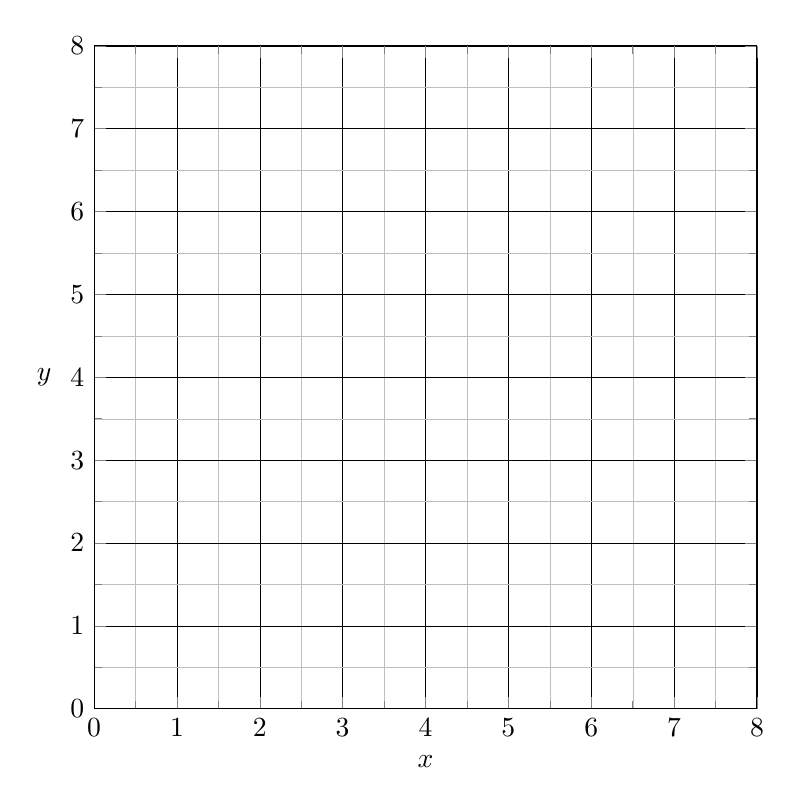
\begin{tikzpicture}
  \begin{axis}[
    xlabel={$x$},
    ylabel={$y$},
    % Rotate the y label by -90 degrees (instead of the default 90°)
    ylabel style={rotate=-90},
    xmin=0, xmax=8,
    ymin=0, ymax=8,
    % Major ticks at integers...
    xtick={0,1,...,8},
    ytick={0,1,...,8},
    % ...and one minor tick between each major tick (i.e. every 0.5)
    minor x tick num=1,
    minor y tick num=1,
    % Draw grid lines at both major and minor ticks
    grid=both,
    % Optional: style the grid lines
    major grid style={line width=0.2pt,draw=black},
    minor grid style={line width=0.1pt,draw=gray!50},
    width=10cm,
    height=10cm,
  ]
    % Add plot commands here if needed.
  \end{axis}
\end{tikzpicture}
\end{document}